% !TEX TS-program = XeLaTeX
% !TEX spellcheck = en-US
\documentclass[aspectratio=169]{beamer}

\usetheme{bi}

\title{Lecture 10:\\ Neural networks II}
\institute{GRA4160: Predictive modelling with machine learning}
\date{March 21rd 2023}
\author{Vegard H\o ghaug Larsen}

\begin{document}

\maketitle

\frame{
	\frametitle{Plan for today:}
	\begin{itemize}
		\item Multilayer neural networks
		\item Optimizers
		\item Weight initialization
		\item Dropout
		\item Convolutional neural networks
	\end{itemize}
}

%\frame{
%	\frametitle{The perceptron}
%}

\frame{
	\frametitle{Multi-layer neural networks}
	\begin{itemize}
		\item A multi-layer neural network is a neural network with more than one hidden layer
		\pause
		\item Modern neural networks typically have more than one hidden layer
		\pause
		%\item The hidden layers are used to learn more complex patterns in the data
		%\pause
		\item The number of hidden layers and the number of hidden units in each layer are hyperparameters that can be tuned
	\end{itemize}
}

\frame{
	\frametitle{Structure of a multilayer neural network}
	\begin{enumerate}
		\item \textbf{Input layer:} This is the first layer of the network, where input features are received. Each neuron in this layer corresponds to a feature from the input data
		\pause
		\item \textbf{Hidden layers:} These are the layers between the input and output layers. They are responsible for learning and extracting higher-level features from the input data. The number of hidden layers and the number of neurons in each hidden layer vary depending on the complexity of the problem
		\pause
		\item \textbf{Output layer:} This is the final layer of the network, responsible for producing the predictions or classification results. The number of neurons in this layer typically depends on the number of target classes or the desired output format
	\end{enumerate}
}

\frame{
	\frametitle{NN with two hidden layers and multiple outputs}
	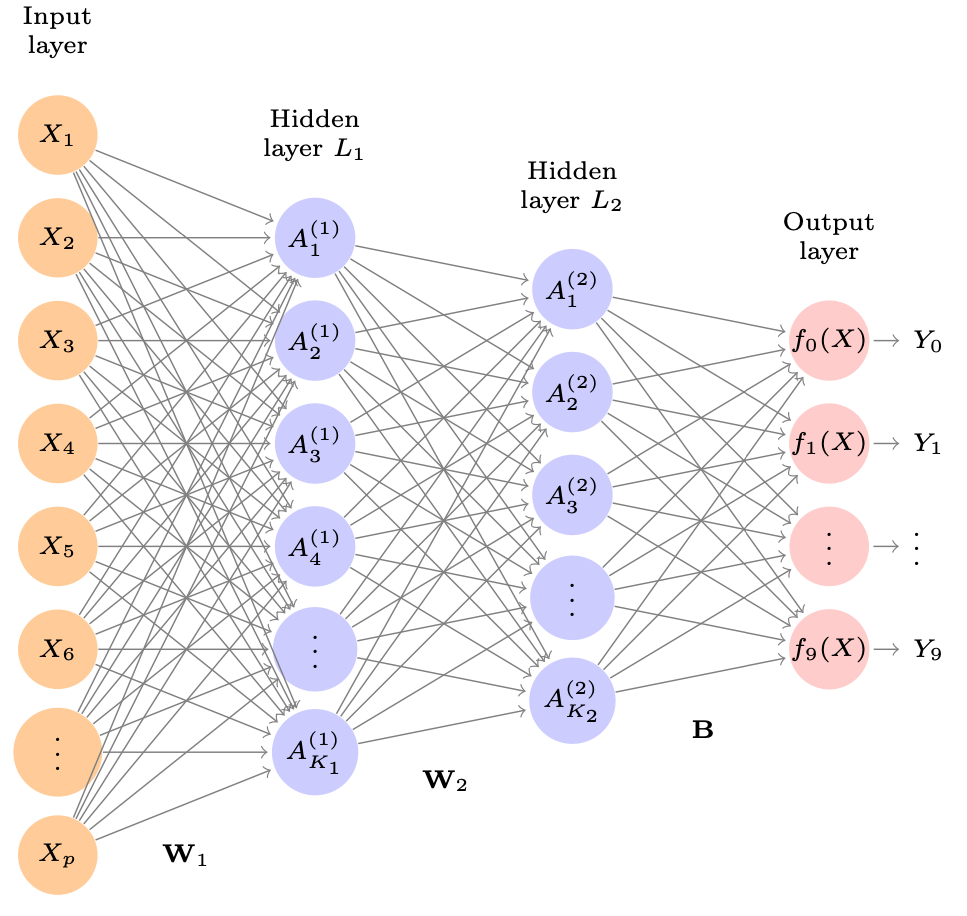
\includegraphics[scale=0.19]{figures/multilayer_NN.png}\\
	{\footnotesize Source: An Introduction to Statistical Learning with Applications in R, James, Witten, Hastie and Tibshirani, 2013}
}

\frame{
  \frametitle{Optimizers}
  \begin{itemize}
    \item \textbf{Gradient Descent}: Updates weights in the direction opposite the gradient, using the entire dataset, which can be computationally intensive for large datasets.
    \pause
    \item \textbf{Stochastic Gradient Descent (SGD)}: Updates weights using a single or small number of samples, leading to faster but noisier convergence.
    \pause
    \item \textbf{Momentum}: Accelerates SGD in the relevant directions and reduces oscillations, improving efficiency in navigating error surfaces.
    \pause
    \item \textbf{Adagrad}: Adapts learning rate for each weight based on past gradients; useful for sparse data but suffers from a continuous decreasing learning rate.
    \pause
    \item \textbf{RMSprop}: Modifies Adagrad by using a moving average of squared gradients, preventing the excessively diminishing learning rates.
    %\pause
    %\item \textbf{Adaptive Moment Estimation (Adam)}: Combines elements from AdaGrad and RMSProp, using adaptive learning rates for each parameter and keeping track of past gradients.
  \end{itemize}
}

\frame{
  \frametitle{Adam Optimizer: Overview}
  \begin{itemize}
    \item \textbf{Introduction}: Adam (Adaptive Moment Estimation) is an optimization algorithm that combines the advantages of two other extensions of stochastic gradient descent, namely AdaGrad and RMSprop.
    \pause
    \item \textbf{Key Concepts}:
      \begin{itemize}
        \item \textit{Adaptive Learning Rates}: Adjusts learning rates based on how frequently a parameter is updated, beneficial for sparse data.
        \item \textit{Moving Averages}: Utilizes the exponential moving averages of both the gradients (first moment) and squared gradients (second moment).
      \end{itemize}
    \pause
    \item \textbf{Mechanism}:
      \begin{enumerate}
        \item Computes the gradients of the loss function with respect to the parameters.
        \item Calculates the exponential moving averages of the gradients and their squares.
        \item Adjusts these averages to correct for their initial bias towards zero.
        \item Updates parameters using these biased-corrected averages, with individual adaptive learning rates.
      \end{enumerate}
  \end{itemize}
}

\frame{
  \frametitle{Adam Optimizer: Continued}
  \begin{itemize}
    \item \textbf{Benefits}:
      \begin{itemize}
        \item \textit{Efficiency}: Requires less memory and is computationally efficient.
        \item \textit{Effective for Large Datasets and Parameters}: Works well with large datasets and high-dimensional parameter spaces.
        \item \textit{Applicability}: Suitable for non-stationary objectives and problems with noisy and/or sparse gradients.
      \end{itemize}
    \pause
    \item \textbf{Hyperparameters}:
      \begin{itemize}
        \item Learning Rate: Typically requires less tuning.
        \item Beta Values: Default values (0.9 for the first moment and 0.999 for the second moment) work well in most cases.
        \item Epsilon: A small constant (like \( 10^{-8} \)) to prevent division by zero.
      \end{itemize}
  \end{itemize}
}

\frame{
  \frametitle{Weight Initialization: An Overview}
  \begin{itemize}
    \item \textbf{Definition}: Weight initialization is the process of setting the initial values of the weights in a neural network before the training process starts.
    \item \textbf{Significance}: The initial weights significantly impact the network's ability to learn efficiently and effectively.
    \item \textbf{Goal}: To start training with weights that neither too small nor too large, avoiding common problems like slow convergence or gradient-related issues.
  \end{itemize}
}

\frame{
  \frametitle{Why Weight Initialization Matters}
  \begin{itemize}
    \item \textbf{Convergence Speed}: Proper initialization leads to a faster convergence by beginning in an advantageous region of the weight space.
    \pause
    \item \textbf{Symmetry Breaking}: Prevents neurons in the same layer from learning identical functions, enhancing the network's ability to learn diverse features.
    \pause
    \item \textbf{Vanishing/Exploding Gradients}: Helps avoid gradients that are too small (vanishing) or too large (exploding), which can hinder learning.
    \pause
    \item \textbf{Local Minima Avoidance}: Randomized initial weights promote exploration of the weight space, reducing the risk of getting trapped in suboptimal local minima.
  \end{itemize}
}

\frame{
  \frametitle{Methods of Weight Initialization}
  \begin{itemize}
    \item \textbf{Zero Initialization}: Initializes all weights to zero, leading to symmetry issues and ineffective learning.
    \pause
    \item \textbf{Random Initialization}: Small random weights using various distributions (uniform or Gaussian) to break symmetry and begin learning.
    \pause
    \item \textbf{Xavier Initialization}: Weights are drawn from a distribution with mean 0 and variance \(\frac{1}{n_{in}}\), ideal for networks with sigmoid or tanh activation functions.
    \pause
    \item \textbf{He Initialization}: Similar to Xavier but with variance \(\frac{2}{n_{in}}\), more suitable for networks with ReLU activation functions.
  \end{itemize}
}

\frame{
  \frametitle{Dropout: A Regularization Technique}
  \begin{itemize}
    \item \textbf{Concept of Dropout}: Introduces randomness into the training process by temporarily removing a subset of neurons (and their connections) in a layer during each training step. This prevents neurons from co-adapting too much.
    \pause
    \item \textbf{Dropout Rate}: Specifies the proportion of neurons to drop out. Common rates range from 0.1 to 0.5, with higher rates imposing stronger regularization effects.
    \pause
    \item \textbf{Impact on Training}: Forces the network to learn more robust and redundant representations, enhancing its ability to generalize well to unseen data.
    \pause
    \item \textbf{Application during Inference}: At inference time, dropout is not applied. Instead, the weights are adjusted to account for the dropout applied during training, maintaining a consistent output scale.
  \end{itemize}
}

\frame{
  \frametitle{Benefits of Implementing Dropout}
  \begin{enumerate}
    \item \textbf{Enhanced Regularization}: Acts as a powerful regularizer by disrupting the co-adaptation among neurons, encouraging the network to develop more generalized features and reducing overfitting.
    \pause
    \item \textbf{Implicit Ensemble Effect}: Simulates training a variety of "thinned" networks with shared weights. The combination of these networks during testing can be viewed as an ensemble method, leading to improved performance and robustness.
    \pause
    \item \textbf{Efficient Training}: By reducing the effective number of neurons during training, Dropout can potentially speed up computations, as there are fewer activations and gradients to propagate.
    \pause
    \item \textbf{Versatility}: Effective across a wide range of neural network architectures and applications, from fully connected layers to convolutional networks.
  \end{enumerate}
}

\frame{
  \frametitle{Introduction to Convolutional Neural Networks (CNNs)}
  \begin{itemize}
    \item \textbf{Purpose}: CNNs are specialized neural networks for processing data with a grid-like topology, such as images, where capturing spatial hierarchies and relationships is crucial.
    \pause
    \item \textbf{Key Characteristics}:
      \begin{itemize}
        \item Optimized for 2D data, particularly effective in handling visual inputs.
        \item Utilize local connectivity and weight sharing to reduce the complexity and increase efficiency.
        \item Exhibit translational invariance, making them robust to the location of features in the input.
      \end{itemize}
    \pause
    \item \textbf{Applications}: Excel in various computer vision tasks, including image and video recognition, image classification, medical image analysis, and many more.
  \end{itemize}
}

\frame{
  \frametitle{Core Components of Convolutional Neural Networks}
  \begin{itemize}
    \item \textbf{Convolutional Layers I}:
      \begin{itemize}
        \item Apply numerous small, learnable filters to capture local patterns such as edges, corners, and textures.
        \item Each filter detects features at different locations, creating a feature map.
      \end{itemize}
    \pause
    \item \textbf{Pooling Layers}:
      \begin{itemize}
        \item Reduce the spatial dimensions (width and height) of the input volume for the subsequent layers.
        \item Enhance feature detection robustness and reduce computational load.
      \end{itemize}
    \pause
    \item \textbf{Fully Connected Layers}:
      \begin{itemize}
        \item After feature extraction and down-sampling, these layers perform high-level reasoning.
        \item Often used at the end of CNNs to classify input into categories based on the extracted features.
      \end{itemize}
  \end{itemize}
}

\frame{
  \frametitle{Convolutional Layers II}
  \begin{itemize}
    \item \textbf{Filter Application}:
      \begin{itemize}
        \item Filters are small matrices that slide over the input, applying a convolution operation.
        \item The convolution emphasizes the presence of specific features at different spatial locations.
      \end{itemize}
    \pause
    \item \textbf{Feature Maps}:
      \begin{itemize}
        \item Each filter produces a feature map, representing the response of the filter at every spatial position.
        \item Multiple filters create a stack of feature maps, forming the output volume.
      \end{itemize}
    \pause
    \item \textbf{Learning Features}:
      \begin{itemize}
        \item Filters are learned during training, enabling the network to identify and respond to various features in the input.
        \item Early layers typically learn basic features (e.g., edges), while deeper layers learn more complex patterns.
      \end{itemize}
  \end{itemize}
}


\frame{
	\frametitle{2D-convolutional layes}
	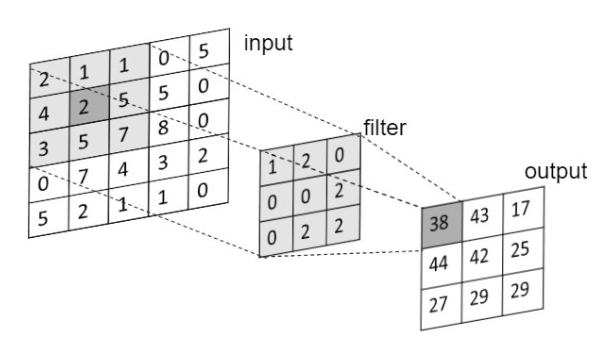
\includegraphics[scale=0.35]{figures/2d_convolution.png}\\
	{\footnotesize Source: Review: Deep Learning on 3D Point Clouds, Bello et al. 2020}

	\[38 = 2\cdot1 + 1\cdot2 + 1\cdot0 + 4\cdot0 + 2\cdot0 + 5\cdot2 + 3\cdot0 + 5\cdot2 + 7\cdot2  \]
}

\frame{
  \frametitle{Pooling Layers: Enhancing Efficiency and Robustness in CNNs}
  \begin{itemize}
    \item \textbf{Function of Pooling Layers}:
      \begin{itemize}
        \item Provide a form of down-sampling, reducing the spatial dimensions (height and width) of the input feature maps.
        \item This process condenses the input into a more manageable form, retaining important features while reducing size.
      \end{itemize}
    \pause
    \item \textbf{Common Pooling Operations}:
      \begin{itemize}
        \item \textit{Max Pooling}: Selects the maximum value from each patch of the feature map covered by the pooling window.
        \item \textit{Average Pooling}: Computes the average of values in each patch, providing a smoothed feature map.
      \end{itemize}
  \end{itemize}
}

\frame{
  \frametitle{Pooling Layers: Continued}
  \begin{itemize}

    \item \textbf{Benefits of Pooling}:
      \begin{itemize}
        \item Enhances the network's translational invariance, making it less sensitive to the exact location of features in the input.
        \item Reduces the computational burden and memory usage by decreasing the number of parameters and computations in the network.
        \item Helps to prevent overfitting by providing an abstracted form of the representation.
      \end{itemize}
    \pause
    \item \textbf{Integration in CNNs}:
      \begin{itemize}
        \item Typically alternated with convolutional layers to progressively reduce the spatial size of the representation and increase the depth of the network.
        \item This structure allows CNNs to efficiently and effectively learn from high-dimensional inputs like images.
      \end{itemize}
  \end{itemize}
}

\frame{
	\frametitle{Architecture of a deep CNN}
	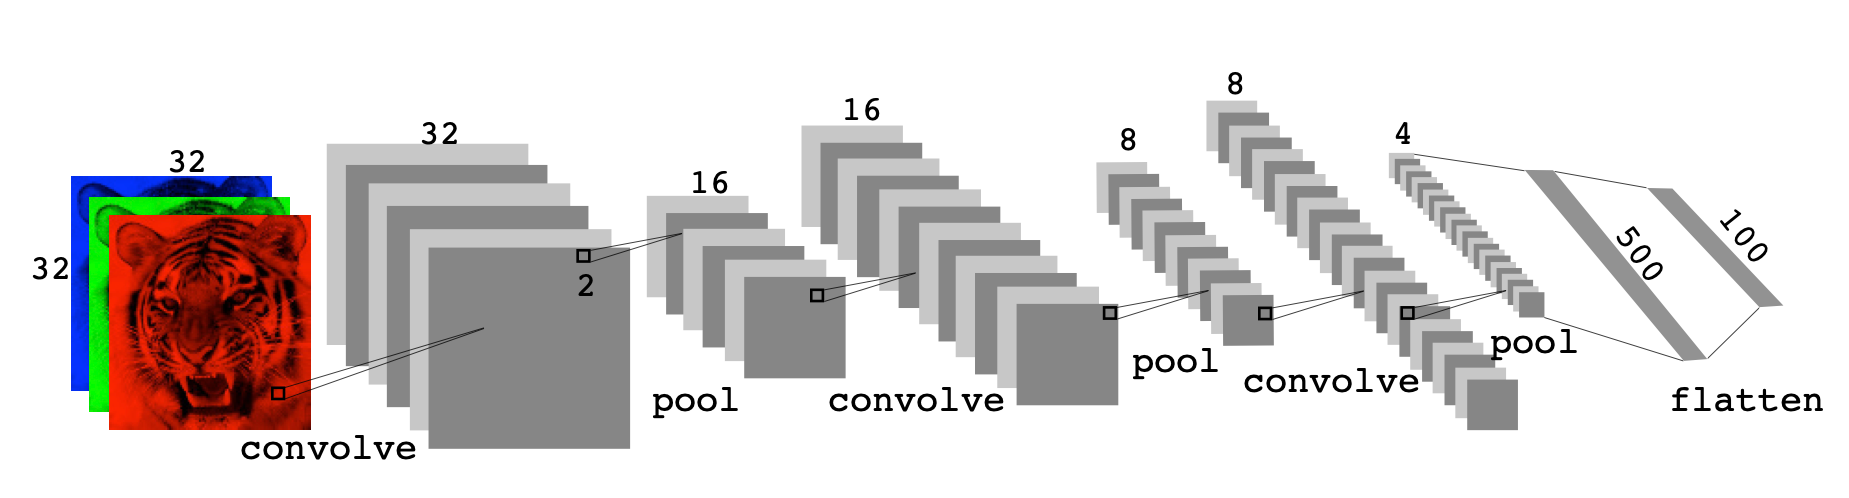
\includegraphics[scale=0.22]{figures/cnn.png}\\
	{\footnotesize Source: An Introduction to Statistical Learning with Applications in R, James, Witten, Hastie and Tibshirani, 2013}
}

\frame{
	\frametitle{Example of pooling}
	Consider a simple $2 \times 2$ input matrix for the pooling operation.
\[
A =
\begin{bmatrix}
a & b \\
c & d
\end{bmatrix}
\]
\pause
Max-pooling selects the maximum value from the input matrix.
\[
\text{max-pooling}(A) = \max(a, b, c, d)
\]
\pause
Average-pooling calculates the average value of the input matrix.
\[
\text{average-pooling}(A) = \frac{a + b + c + d}{4}
\]
}

\frame{
	\frametitle{Max-pooling and average-pooling}
\[ B =
\begin{bmatrix}
7 & 3 & 5 & 2 \\
2 & 8 & 4 & 7 \\
4 & 3 & 5 & 2 \\
3 & 2 & 4 & 5 \\
\end{bmatrix}
\]

\[ \text{max-pooling}(B) =\begin{bmatrix}
8 & 7 \\
4 & 5
\end{bmatrix},\;\;\;\; \text{average-pooling}(B) = \begin{bmatrix}
5 & 4.5 \\
3 & 4
\end{bmatrix} \]
}

%\frame{
%	\frametitle{Batch normalization}
%}

%\frame{
%	\frametitle{Padding}
%}

\end{document}

Introduction to Multilayer Neural Networks

Multilayer neural networks, also known as deep neural networks, consist of multiple layers of interconnected neurons arranged between the input and output layers. The layers between the input and output layers are called hidden layers. Each hidden layer can be seen as a transformation or feature extraction process that helps the network learn complex patterns from the input data.

Structure of a Multilayer Neural Network

Input layer: This is the first layer of the network, where input features are received. Each neuron in this layer corresponds to a feature from the input data.
Hidden layers: These are the layers between the input and output layers. They are responsible for learning and extracting higher-level features from the input data. The number of hidden layers and the number of neurons in each hidden layer vary depending on the complexity of the problem.
Output layer: This is the final layer of the network, responsible for producing the predictions or classification results. The number of neurons in this layer typically depends on the number of target classes or the desired output format.
Activation Functions

Activation functions play a critical role in multilayer neural networks. They introduce nonlinearity into the network, allowing it to learn complex and nonlinear patterns from the data. Common activation functions include the sigmoid, hyperbolic tangent (tanh), and rectified linear unit (ReLU).

Advantages of Multilayer Neural Networks

Representation learning: Multilayer neural networks can automatically learn useful representations and features from raw data, reducing the need for manual feature engineering.
Nonlinear modeling: Due to the presence of activation functions, these networks can model complex, nonlinear relationships between inputs and outputs.
Universality: Multilayer neural networks are universal function approximators, meaning they can approximate any continuous function, given a sufficient number of neurons and layers.
Scalability: Deep learning frameworks make it relatively easy to scale and train large neural networks on massive datasets using parallel and distributed computing.
Challenges

While multilayer neural networks offer numerous benefits, they also come with challenges, including:

Training complexity: Deeper networks with many layers require more computational resources and time to train.
Overfitting: Networks with a large number of parameters are prone to overfitting, especially when dealing with limited or noisy training data.
Interpretability: Understanding the internal workings of a multilayer neural network can be challenging, making it difficult to explain the reasoning behind their predictions.
Vanishing/exploding gradients: During training, gradients can become very small (vanish) or very large (explode), leading to slow convergence or instability.
In summary, multilayer neural networks provide a powerful tool for tackling complex machine learning tasks. By combining multiple layers of neurons with nonlinear activation functions, these networks can learn hierarchical representations of input data and model intricate relationships. However, they also come with challenges that researchers and practitioners must address to ensure successful implementation.